\documentclass{article}
\usepackage[utf8]{inputenc}
\usepackage{amsmath,amssymb}
\usepackage[left=2.5cm,right=2.75cm,bottom=3.5cm,top=2.5cm]{geometry}
\usepackage{tikz-cd}
\usepackage[utf8]{inputenc}
\usepackage[spanish]{babel}
\usetikzlibrary{cd}
\usepackage{amsthm}
\usepackage{stmaryrd}
\usepackage[dvips,all]{xy}
\usepackage{mathtools}

\newtheorem{theorem}{Teorema}
\newtheorem{exercise}{Ejercicio}
\newtheorem{solution}{Resolución}
\newtheorem{example}{Ejemplo}
\newtheorem{lemma}{Lema}
\newtheorem{proposition}{Proposition}

\def\Q{\mathbb{Q}}
\def\R{\mathbb{R}}
\def\I{[a,b]} 
% Esto sirve para abreviar comandos que uno usa con frecuencia y así tener que tipear menos. El comando para hacer la Q de los racionales es \mathbb{Q}; con esta línea, yo le digo a LaTeX que de ahora en más \Q va a significar eso mismo. %

\parskip 0.5em
% El espacio entre párrafos. %

\title{Métodos numéricos para encontrar puntos fijos}
\author{Guillermo Mosse}

\begin{document}

\maketitle

Repaso: Hoy vamos a buscar puntos fijos, es decir, valores de x tal que $f(x)=x$.

¿Para qué sirven? 

Quiero $r$ raíz $f$, es decir, tal que $f(r)=0 \Rightarrow$ Puedo buscar $r$ punto fijo de $g(x) = x + f(x)$ (¡también sirven otras $g$!)

Quiero $r$ punto fijo de $g$, es decir, tal que $g(r)=r \Rightarrow$ Puedo buscar $r$ raíz de $f(x) = g(x) - x$

Esto me permite pasar de un problema a otro.

Además, la existencia y unicidad de puntos fijos de una función atraviesa la matemática, habiendo ejemplos en lógica, computabilidad, geometría, álgebra, etc. 

Algunas aplicaciones:

\begin{itemize}
    \item En el teorema de Picard–Lindelöf (el teorema que garantiza existencia y unicidad de ecuaciones diferenciales de primer orden con condiciones iniciales dadas) se usa un teorema que garantiza existencia de punto fijo en la demostración.
    \item El teorema de la función inversa se puede demostrar usando el teorema de punto fijo de Banach.
    \item En problemas de optimización, la búsqueda de mínimos locales se corresponde a veces con la búsqueda de puntos fijos de funciones.
    \item Muchos algoritmos terminan cuando llegan a un punto fijo, luego garantizar que existe un punto fijo + una propiedad del algoritmo (monocicidad) es garantizar que el algoritmo termina
    \item El desarrollador de Teoría de Juegos, Nash, demostró la existencia de los equlibrios de Nash en cierto tipo de juegos usando un teorema de existencia de punto fijo. Le dieron el premio Nóbel de economía en parte por ese trabajo.
\end{itemize}


\begin{theorem}Sea $g :[a,b] \rightarrow \R\text{ tal que }|g(x)-g(y)|\leq k |x-y|\ \forall\ x,y\ \in [a,b]$ con $0<k<1$ y además $g([a,b]) \subset [a,b]$. \\

Entonces $g$ tiene un único punto fijo $r \in [a,b]$ y es límite de la sucesión

\begin{equation}
  \left\{
  \begin{array}{@{}ll@{}}
    x_0 \in [a,b] \text{ arbitrario} \\
    x_{n+1} = g(x_n)
  \end{array}\right.
\end{equation} 

Además, $\forall\ n$ se tiene $|x_n-r| \leq \frac{k^n}{1-k} |x_1-x_0|$ y también $|x_n-r|\leq k^n \underbrace{|x_0 -r|}_{\leq b-a}$ \\

Observación: La primera desigualdad nos permite acotar el error en función de algo fácilmente calculable.

\end{theorem} 




\begin{theorem}  Sea  $g :[a,b] \rightarrow \R$ es $C^1$ en $(a,b)$ y $r\in(a,b)$ un punto fijo de $g$. Si $|g'(r)|<1$ entonces $\exists\ \varepsilon>0$ tal que la iteración de antes es convergente siempre que $x_0 \in (r-\varepsilon,r+\varepsilon)$
\end{theorem} 

Observación: en la práctica vamos a probar que $g' < 1$ en un intervalito donde sabemos que hay un punto fijo porque no sabemos \textit{cuál} es el punto fijo.


\begin{exercise}
Sea $f(x)=2^{-x}-x$.

\[
\begin{rcases*}
f(1/3) > 0 \\
f(1) < 0
\end{rcases*} \text{Por Bolzano, hay raíz en } (\frac{1}{3},1)
\]

Busquemos la raíz con un método de punto fijo.

Propongo $g(x) = 2^{-x}$
$$g(x) = x \Leftrightarrow f(x)=0$$ (sale de pedir $f(x)=0$ e intentar despejar la x en función de alguna expresión y llamarla $g$. ¡Puede haber más de una $g$!)



¿Cumple $g(x)$ las condiciones del teorema?

Veamos que $\forall\ x,y\in (\frac{1}{3},1)$, vale que $|g(x)-g(y)| \leq k |x-y|$, con $k < 1$, es decir, que g es Lipschitz en ese intervalo con una constante menor que 1.

Derivemos y usemos el TVM, una gran herramienta:

$g'(x)=-ln(2)\ e^{-x\ ln(2)} = - ln(2)\ 2^{-x}$

Luego $|g'(x)| \leq ln(2)\ 2^{-x} \underset{x > 0}{\leq} ln(2) < 1$

Entonces, por el TVM,  $\forall\ x,y\in (\frac{1}{3},1)$,$|g(x)-g(y)|\ \leq ln(2) |x-y|$

¿Cómo podemos ver que g del intervalo queda dentro del intervalo?

$$g(1/3) < 1$$
$$g(1) > 1/3$$

y además $g$ es decreciente. Luego $g([\frac{1}{3},1]) \subset [\frac{1}{3},1])$. ¡Graficar la función $g$ para convencerse!

Luego, la iteración es convergente.

¿Cuántos pasos debo hacer para obtener un error menor que $10^{-8}$? \bigskip

$|x_n-r| \leq \frac{k^n}{1-k} |x_1-x_0| \leq \frac{ln(2)^n}{1-ln(2)} \frac{2}{3} < 10^{-8} \rightarrow$ y busco n.

%¿Cuál es el orden de convergencia?

%$|x_{n+1} - r| = |g(x_n) - g(r)| \underset{TVM}{=} | g'(\chi_n) | |x_n - r|$
 
%Luego $\frac{|x_{n+1} - r|}{|x_n - r|} = |g'(\chi_n)| |x_n-r| \xrightarrow[n \to \infty]{} ln(2) 2^{-r} \neq 0$. Entonces el orden es exactamente 1.

Entendamos más geométricamente qué está haciendo este algoritmo.

 Gráfico del algoritmo aplicado a una función parecida a $g(x)$: \\
 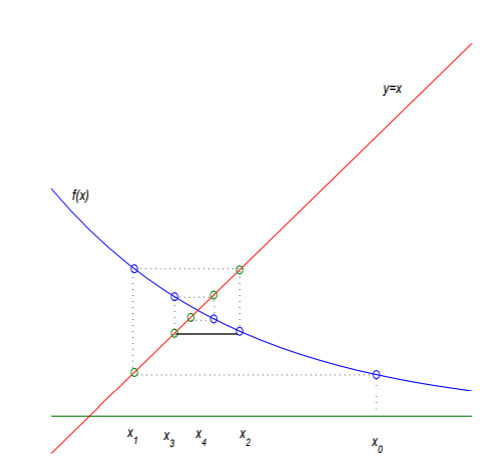
\includegraphics{PuntoFijoEjemplo.png}
 
 (En clase lo haremos con más detalles, si Rossi no lo hizo ya)
\end{exercise}


\begin{exercise}
    A veces hay que tener cuidado al pasar de la $f$ a la que le buscamos una raíz a la $g$ a la que le buscamos un punto fijo. Veámoslo en el siguiente ejercicio (de parcial): \\
    
    Sea $f(x)= ln(x) + x$. Se sabe que tiene una única raíz en $I= [1/2,1]$. ¿Qué función g(x) y qué intervalo se pueden usar para armar una iteración convergente del algoritmo de punto fijo?
    
    Resolución: se pueden armar las siguientes funciones g(x), por ejemplo: \bigskip
    
    $$g_1(x)=-ln(x),\ g_2(x)=e^{-x},\ g_3(x) = \frac{x+e^{-x}}{2}$$
    
    Ejercicio: verificar $g_i(x) = x \Leftrightarrow f(x) = 0$
    
    1) $g_1(x) = -ln(x)$
    $g_1'(x)=\frac{-1}{x}$\\
    $$|\frac{-1}{x}| = \frac{1}{x} \underset{x \geq 1/2}{\geq} 1 \rightarrow \text{ No es contracción así que no sirve.} $$
    
    
    2) $g_2(x) = e^{-x}$
    $$|g_2'(x)| = |-e^{-x}| = e^{-x} \leq \frac{1}{\sqrt{e}} < 1 \rightarrow \text{¡es contracción!}$$
    
    ...pero $g(I) \not\subset I$, pues $g(1) < 1/2$.
    
    ¿Cómo se arregla esto? Cuánto más chico sea el intervalo donde sabemos que hay un punto fijo de $g$/raíz de $f$, mejor (es más fácil cumplir las hipótesis de los teoremas en un subintervalo de $I$ que en $I$).
    
    Luego, podemos hacer bisección, a mano, por ejemplo.
    
    Tomo $[\frac{1}{2},\frac{3}{4}]$ ó $[\frac{3}{4},1]$ \\
    
    $f(3/4) > 0, f(1/2) < 0$ así que tomamos $I_2 = [\frac{1}{2},\frac{3}{4}]$
    
    Ejercicio: $I_2$ no alcanza porque $g_2(I_2) \not\subset I_2$.  Pero siguiendo dos veces más con bisección  llegamos a que $I_4 = [0,5;0.5625]$ sí.
    
    ¿Hace falta ver que es contracción en ? $I_3$¡No! Porque estamos en un subintervalo. \bigskip
    
    En $g_3$ va a estar todo bien, pero es más galerazo.
    
    
    
    %TODO: hacer un gráfico.
\end{exercise}


\begin{exercise}
    Veamos gráficamente qué pasa cuando no se cumplen las hipótesis: sea $f(x) = x^2-2x-3$. \\
    
    Sea $g(x) = \frac{x^2-3}{2}$. Esta función no cumple ninguna de las dos hipótesis, y $x_n \xrightarrow[n \to \infty]{} \infty$. Hacer gráfico y ver cómo se van moviendo los $x_n$.\\
    
    Observación: aunque no se cumplan las hipótesis de los teoremas, eso no quiere decir que el algoritmo no converja. Exploremos eso un poquito en el siguiente ejercicio.
\end{exercise}



\begin{exercise}
    Sea $f(x) = x^2-x-2 \rightarrow \text{Propongo }g(x) = \sqrt{x+2}$
    
    Observación: si el algoritmo converge, lo hará a una raíz positiva de $f$. \bigskip
    
    $$g'(x) = \frac{1}{2\sqrt{x+2}} > 0 \Rightarrow $$
    
    $$\frac{1}{2\sqrt{x+2}} < 1 \Leftrightarrow 1 < 2 \sqrt{x+2} \Leftrightarrow  x > -7/4$$
    
    ¿Sirve $I = [-7/4,+\infty)$? $g(I) \subset I$ pues $g \geq 0$ pero $g'(-7/4) = 1$ y nosotros no queremos eso. Si achico un poco el intervalo, por ejemplo, si tomo $I_2 = [0, +\infty]$, ahí $g'(x) \leq g'(0) = \frac{1}{2\sqrt{2}} < 1$.
    
    ¿Hace falta chequear $g(I_2) \subset I_2$? \textbf{Sí}. (¡Pensar por qué esta vez sí!)
    
    ¿Pero es este el intervalo maximal que puedo tomar?
    
$Dom\ g = [-2,+\infty)$. Si tomo $x \in [-2,0], g(x) \in [0, +\infty)$. Y sabemos que en ese intervalo la cosa anda, así que el intervalo maximal de convergencia resulta ser tooodo el dominio de $g$. ¡Qué bueno!
\end{exercise}

\begin{exercise}

Para pensar: sea $f(x)$ una función continua, $x_0 \in \R$ y definamos $x_{n+1} = f(x_n)$.

Supongamos que la sucesión $x_n$ es convergente. Probar que necesariamente debe converger a un punto fijo de $f$.

\end{exercise}



\end{document}